\documentclass[12pt,utf8,notheorems,compress,t]{beamer}
\usepackage{etex}

\usepackage{pgfpages}
\usepackage[export]{adjustbox}

% Workaround for the issue described at
% https://tex.stackexchange.com/questions/164406/beamer-using-href-in-notes.
\newcommand{\fixedhref}[2]{\makebox[0pt][l]{\hspace*{\paperwidth}\href{#1}{#2}}\href{#1}{#2}}

\usepackage[english]{babel}

\usepackage[normalem]{ulem}
\usepackage{graphbox}
\usepackage{mathtools}
\usepackage{booktabs}
\usepackage{stmaryrd}
\usepackage{amssymb}
\usepackage{array}
\usepackage{ragged2e}
\usepackage{multicol}
\usepackage{tabto}
\usepackage{xstring}
\usepackage{proof}
\usepackage{ifthen}
\usepackage[normalem]{ulem}
\usepackage[all]{xy}
\xyoption{rotate}
\usepackage{tikz}
\usetikzlibrary{calc,shapes,shapes.callouts,shapes.arrows,patterns,fit,backgrounds,decorations.pathmorphing,positioning,svg.path}
\hypersetup{colorlinks=true}

\newcommand*\circled[1]{\tikz[baseline=(char.base)]{%
  \node[shape=circle,draw,inner sep=1pt] (char) {#1};}}

\DeclareFontFamily{U}{bbm}{}
\DeclareFontShape{U}{bbm}{m}{n}
   {  <5> <6> <7> <8> <9> <10> <12> gen * bbm
      <10.95> bbm10%
      <14.4>  bbm12%
      <17.28><20.74><24.88> bbm17}{}
\DeclareFontShape{U}{bbm}{m}{sl}
   {  <5> <6> <7> bbmsl8%
      <8> <9> <10> <12> gen * bbmsl
      <10.95> bbmsl10%
      <14.4> <17.28> <20.74> <24.88> bbmsl12}{}
\DeclareFontShape{U}{bbm}{bx}{n}
   {  <5> <6> <7> <8> <9> <10> <12> gen * bbmbx
      <10.95> bbmbx10%
      <14.4> <17.28> <20.74> <24.88> bbmbx12}{}
\DeclareFontShape{U}{bbm}{bx}{sl}
   {  <5> <6> <7> <8> <9> <10> <10.95> <12> <14.4> <17.28>%
      <20.74> <24.88> bbmbxsl10}{}
\DeclareFontShape{U}{bbm}{b}{n}
   {  <5> <6> <7> <8> <9> <10> <10.95> <12> <14.4> <17.28>%
      <20.74> <24.88> bbmb10}{}
\DeclareMathAlphabet{\mathbbm}{U}{bbm}{m}{n}
\SetMathAlphabet\mathbbm{bold}{U}{bbm}{bx}{n}

\usepackage{pifont}
\newcommand{\cmark}{\ding{51}}
\newcommand{\xmark}{\ding{55}}
\DeclareSymbolFont{extraup}{U}{zavm}{m}{n}
\DeclareMathSymbol{\varheart}{\mathalpha}{extraup}{86}

\graphicspath{{images/}}

\usepackage[protrusion=true,expansion=true]{microtype}

\setlength\parskip{\medskipamount}
\setlength\parindent{0pt}

\title{On the scope of the dynamical method in commutative algebra}

\author{Ingo Blechschmidt}
\date{January 18th, 2022}

%\useinnertheme[shadow=true]
\setbeamerfont{block title}{size={}}

\useinnertheme{rectangles}

\usecolortheme{orchid}
\usecolortheme{seahorse}
\definecolor{mypurple}{RGB}{253,73,34}
\definecolor{mypurpledark}{RGB}{100,0,150}
\setbeamercolor{structure}{fg=mypurple}
\definecolor{myred}{RGB}{150,0,0}
%\setbeamercolor*{title}{bg=myred,fg=white}
%\setbeamercolor*{titlelike}{bg=myred,fg=white}
\setbeamercolor*{title}{bg=mypurple,fg=white}
\setbeamercolor*{titlelike}{bg=mypurple,fg=white}
\setbeamercolor{frame}{bg=black}

\usefonttheme{serif}
\usepackage[T1]{fontenc}
\usepackage{libertine}

% lifted from https://arxiv.org/abs/1506.08870
\DeclareFontFamily{U}{min}{}
\DeclareFontShape{U}{min}{m}{n}{<-> udmj30}{}
\newcommand\yon{\!\text{\usefont{U}{min}{m}{n}\symbol{'210}}\!}

\newcommand{\A}{\mathcal{A}}
\newcommand{\B}{\mathcal{B}}
\newcommand{\C}{\mathcal{C}}
\newcommand{\M}{\mathcal{M}}
\renewcommand{\AA}{\mathbb{A}}
\newcommand{\BB}{\mathbb{B}}
\newcommand{\pp}{\mathbbm{p}}
\newcommand{\MM}{\mathbb{M}}
\newcommand{\E}{\mathcal{E}}
\newcommand{\F}{\mathcal{F}}
\newcommand{\FF}{\mathbb{F}}
\newcommand{\G}{\mathcal{G}}
\newcommand{\J}{\mathcal{J}}
\newcommand{\GG}{\mathbb{G}}
\renewcommand{\O}{\mathcal{O}}
\newcommand{\K}{\mathcal{K}}
\newcommand{\NN}{\mathbb{N}}
\newcommand{\QQ}{\mathbb{Q}}
\newcommand{\RR}{\mathbb{R}}
\newcommand{\TT}{\mathbb{T}}
\newcommand{\PP}{\mathbb{P}}
\newcommand{\ZZ}{\mathbb{Z}}
\newcommand{\CC}{\mathbb{C}}
\renewcommand{\P}{\mathcal{P}}
\newcommand{\aaa}{\mathfrak{a}}
\newcommand{\ccc}{\mathfrak{c}}
\newcommand{\ppp}{\mathfrak{p}}
\newcommand{\fff}{\mathfrak{f}}
\newcommand{\mmm}{\mathfrak{m}}
\newcommand{\defeq}{\vcentcolon=}
\newcommand{\defeqv}{\vcentcolon\equiv}
\newcommand{\Sh}{\mathrm{Sh}}
\newcommand{\GL}{\mathrm{GL}}
\newcommand{\Zar}{\mathrm{Zar}}
\newcommand{\op}{\mathrm{op}}
\newcommand{\Set}{\mathrm{Set}}
\newcommand{\Eff}{\mathrm{Ef{}f}}
\newcommand{\Sch}{\mathrm{Sch}}
\newcommand{\Aff}{\mathrm{Aff}}
\newcommand{\Ring}{\mathrm{Ring}}
\newcommand{\LocRing}{\mathrm{LocRing}}
\newcommand{\LRS}{\mathrm{LRS}}
\newcommand{\Hom}{\mathrm{Hom}}
\newcommand{\Spec}{\mathrm{Spec}}
\newcommand{\lra}{\longrightarrow}
\newcommand{\RelSpec}{\operatorname{Spec}}
\renewcommand{\_}{\mathpunct{.}}
\newcommand{\?}{\,{:}\,}
\newcommand{\speak}[1]{\ulcorner\text{\textnormal{#1}}\urcorner}
\newcommand{\ul}[1]{\underline{#1}}
\newcommand{\affl}{\ensuremath{{\ul{\ensuremath{\AA}}^1}}}
\newcommand{\Ll}{\text{iff}}
\newcommand{\inv}{inv.\@}
\newcommand{\seq}[1]{\mathrel{\vdash\!\!\!_{#1}}}
\newcommand{\hg}{\mathbin{:}}  % homogeneous coordinates

\setbeamertemplate{blocks}[rounded][shadow=false]

\newenvironment{indentblock}{%
  \list{}{\leftmargin\leftmargin}%
  \item\relax
}{%
  \endlist
}

% Adapted from https://latex.org/forum/viewtopic.php?t=2251 (Stefan Kottwitz)
\newenvironment<>{hilblock}{
  \begin{center}
    \begin{minipage}{9.05cm}
      \setlength{\textwidth}{9.05cm}
      \begin{actionenv}#1
        \def\insertblocktitle{}
        \par
        \usebeamertemplate{block begin}}{
        \par
        \usebeamertemplate{block end}
      \end{actionenv}
    \end{minipage}
  \end{center}}

\newenvironment{changemargin}[2]{%
  \begin{list}{}{%
    \setlength{\topsep}{0pt}%
    \setlength{\leftmargin}{#1}%
    \setlength{\rightmargin}{#2}%
    \setlength{\listparindent}{\parindent}%
    \setlength{\itemindent}{\parindent}%
    \setlength{\parsep}{\parskip}%
  }%
  \item[]}{\end{list}}

\tikzset{
  invisible/.style={opacity=0,text opacity=0},
  visible on/.style={alt={#1{}{invisible}}},
  alt/.code args={<#1>#2#3}{%
    \alt<#1>{\pgfkeysalso{#2}}{\pgfkeysalso{#3}}}
}

% https://tex.stackexchange.com/questions/172336/drawing-roman-laurel-leaves-spqr-in-tikz
\tikzset{
  laurel-wreath/.pic = {
    \fill svg{M14.4-24.6c-1.5-1.5-2.6-3.3-3.1-5.3l-.4-1.7c-.2-1.1-.2-4.1 .2-5.7 .2-.9 .3-1.3 .5-1.3l1.4 1.1 2.5 2.4c2.7 2.5 5.2 6 5.8 8 .2 .6-.5 .3-2.2-.9-1.6-1.3-3.3-2.6-5-3.8l.1 1.4c.2 1.4 .5 2.7 1.1 4.6s.8 2.5 .5 2.5l-1.4-1.3zm69.6 1.1 .3-1.2c.8-2.3 1.3-4.8 1.6-7.3l-1.5 1.1c-1.3 .9-2.6 1.9-3.7 3-1.6 1.1-2 1.3-2.1 1 .7-1.8 1.6-3.4 2.8-4.9 1.3-1.7 6.5-6.8 7-6.8 .2 0 .3 .2 .3 .5l.3 1.6c.3 2.2 .2 5.7-.5 7.4-.8 1.9-1.6 3.1-3 4.7-1.1 1.1-1.4 1.3-1.5 .9z};
    \fill svg{M10-29.4c-.8-1.1-1.4-2.2-2-4.1l-.7-3.5c-.2-3 .2-4.4 1.4-8.3l.5-1.4c.2-1.3 .3-1.9 .6-1.9 .3-.2 .6 .3 .7 .8s.9 2.2 1.9 3.6c1.4 2.2 2.7 4.4 3.9 6.6l.9 2.7c0 .6 0 .6-.3 .6-.6 0-4.9-4.4-5.8-6l-.2-.6-.1 1.7-.3 2.8c-.3 2.7-.3 3.8 0 5.5 .6 2 .5 2.4-.5 1.5zm79.2 .3 .4-2.4c.2-1.3 .2-2.7-.1-4.9l-.3-2.8v-1.6l-.7 1c-.8 1.3-5 5.5-5.5 5.5s-.5-.3 .2-1.9c.5-1.7 1.4-3.3 3.3-6.5 2.4-3.6 2.7-3.9 2.8-4.7 .5-1.3 .5-1.4 .8-1.2 .3 0 .6 .8 .6 1.5l.7 2.4c.9 2.7 1.1 3.6 1.2 6 .2 3.1-.5 6-2 8.2-.8 1.3-1.3 1.7-1.4 1.5z};
    \fill svg{M5-40c-.4-3.2-.1-6.5 .9-9.6 .5-1.1 1.6-2.8 2.2-3.4l1.3-1.6 2-2.7 .2 .6c.1 1.3 .4 2.6 .9 3.8l.3 1c.8 1.7 1.1 2.7 1.6 5.3 .6 2.5 .6 4.6 .2 4.6-.3 0-.9-.8-1-1.1l-.5-.8c-1.4-2-3-5.2-2.9-6.5-.9 2.7-2 5.4-3.5 7.9l-.3 .8-.3 .8c0 .5-.6 1.6-.8 1.6l-.3-.7zm89.2 .2-.2-.5-.3-.9-1.1-2.7-1.1-2.4c-.6-1.4-1.2-2.8-1.6-4.2l-.3 .9c-.3 1.3-1.6 3.9-3 6-1.3 2-1.6 2-1.5 0s1.1-6.3 2.2-9c.8-1.7 1.1-3.1 .9-4.1-.2-1.1 .5-.8 2.2 1.8 3.3 4.4 3.8 5.4 4.4 7.8 .6 2.4 .5 7.7-.3 7.8l-.3-.5z};
    \fill svg{M13.9-50.1c-.5-1.9-.8-3.9-.9-5.8-.2-1.6-.1-3.3 .1-4.9-.3 .8-1.7 2.5-4.2 5.1l-3 4.9-.3 .1c-.3 0-.3-2.2 0-3.3 .8-3 1.4-4.6 2.5-6.1 .9-1.3 1.7-1.9 2.5-2.5 1.1-.6 2.7-1.9 3.5-2.7 .9-.9 1.9-1.4 2.2-1.4v1.1l-.3 6.6c0 6.8 .2 6.3-1 8.9-.5 1.1-.8 1.1-1.1 0zm70.8-.4c-.8-2.2-.8-2.5-.7-6.3-.1-2.7-.1-5.5-.2-8.2-.3-1.6-.3-1.9 .5-1.6l.6 .5c1.4 1.4 3 2.5 3.9 3.1 1.3 .9 1.9 1.6 2.7 2.6l.6 .7 .2 .4 .2 .3c.8 .9 2 4.9 2 6.9 .2 1.9-.2 1.9-.9 .5-.7-1.4-1.5-2.7-2.6-4-1.6-1.5-3-3.2-4.2-5 .4 3 .3 6-.5 9 0 .8-.5 2.2-.8 2.3-.2 0-.5-.3-.8-1.2z};
    \fill svg{M16.4-58.5l.2-1.5 .3-3.7c.2-2.8 .3-3.5 1.1-5.4l.7-1.3-.5 .4-1 .7c-.5 .4-1.1 .8-1.5 1.3l-.5 .3-1.9 1.6c-2.2 1.6-2.7 2-3.9 3.6-.5 .8-1.1 1.3-1.3 1.3-.5 0 0-2.4 1.1-4.7 1.5-3.4 4.3-6 7.7-7.4l1.3-.4 1.9-.4 2-.5c1.4 0 1.4 0 1 1.1-.5 .8-.8 2-1.1 4.2-.3 2.3-1.1 4.5-2.2 6.5l-.4 .6c-.6 1.1-1.3 2.1-2 3.2-.5 .6-.8 .8-1 .5zm66.3-.2c-.8-.9-2.8-4.4-3.5-6.1-.6-1.3-.9-2.5-1.1-3.5-.2-2.1-.7-4.1-1.5-6 0-.3 0-.3 1.2-.3l2.1 .5 1.9 .4 1.2 .4 .6 .1 1 .6c3 1.4 5.7 4.6 6.8 8.5l.7 2.6c-.2 .6-.5 .5-1.4-.7-2.2-2.7-4.8-5-7.7-6.9l-1.7-1.3 .6 1.3c.3 .6 .6 1.2 .8 1.9l.3 2.5 .3 3.9c.3 2.4 .2 2.8-.6};
    \fill svg{M21.6-66.1l.4-1.1 .9-3.2c.3-1.9 1.1-3.3 2.4-4.7l.4-.8-1.2 .2-2.2 .3c-2.7 .3-5.3 1.2-7.7 2.5-.6 .5-1.3 .6-1.3 .3 0-.5 .9-1.9 2-2.9 .8-.9 2-1.9 3.2-2.6l.9-.4 2.2-1c.3-.2 1.3-.3 3.2-.1 3 0 4.1 .2 6.3 .7l1.1 .4c.5 .2 .6 .6 .3 .6-.5 0-1.4 .9-1.9 1.7l-1.2 1.8c-1.7 2.8-2.2 3.5-4.6 5.9l-3 2.7-.2-.3zm53.9-2c-2.7-2.8-3.5-3.8-5.4-6.8-.9-1.6-1.4-2.4-1.9-2.5l-.8-.5c-.3 0-.2-.5 .4-.6l1.1-.4c1.9-.6 3-.8 5.6-.9l3.3 .2c2 .6 3.8 1.5 5.4 2.8 .3 0 1.9 1.6 2.5 2.4l.9 1.8c0 .3-.3 .2-1.9-.6-2.8-1.4-4.4-1.9-7.7-2.2l-2.2-.5c-.9-.2-.9-.2-.6 .2 .6 .5 1.7 2 2.1 2.8l.9 2.5c.3 1.5 .6 3 .9 4.6l-2.6-2.3z};
    \fill svg{M34.1-78.7c-3.4-1.3-6.9-2.1-10.6-2.5-.9 0-1.4 0-2.3 .3-2 .5-2 0 0-1.3l2.8-1.2c1.4-.5 1.9-.5 3.8-.6 3.8-.2 6.1 .3 9.3 1.7l3.6 1.1 2.2 .3c1.3 0 1.7 0 2.7-.3 1.1-.3 2.8-1.1 2.8-1.3l-1.3-.9c-1.9-1.4-3.1-2.7-3.1-3.2l.8-.6c.9-.3 1.3-.2 2 .8 .5 .8 1.1 1.4 2.9 2.7 .2 .3 .3 .2 1.1-.3 .9-.8 2.4-2 2.6-2.7 .5-.6 .9-.8 1.8-.5l.8 .6c0 .5-1.4 1.7-3.2 3.2l-1.3 .9c0 .2 1.7 .9 2.9 1.3 .9 .3 1.4 .3 2.7 .3l2.2-.3c1.7-.4 3.4-1 5-1.7 2-.8 4.4-1.3 7.7-1.1 2 .2 2.5 .2 3.8 .6 .9 .3 2.2 .8 2.8 1.2 2 1.1 2 1.6 .2 1.3-1.6-.3-1.9-.3-4.4 0-2.4 .3-4.7 .8-7 1.6l-1.5 .6c-2.9 .3-5.9 .2-8.8-.3-1.7-.3-3.6-.9-6-2.1l-1.1-.4-1.3 .6c-4.5 2.2-9.6 3-14.6 2.2zm-6.3-9.1c};
  }
}

\newcommand{\pointthis}[3]{%
  \tikz[remember picture,baseline]{
    \node[anchor=base,inner sep=0,outer sep=0] (#2) {#2};
    \node[visible on=#1,overlay,rectangle callout,rounded corners,callout relative pointer={(0.3cm,0.5cm)},fill=blue!20] at ($(#2.north)+(-0.1cm,-1.1cm)$) {#3};
  }%
}

\tikzset{
  invisible/.style={opacity=0,text opacity=0},
  visible on/.style={alt={#1{}{invisible}}},
  alt/.code args={<#1>#2#3}{%
    \alt<#1>{\pgfkeysalso{#2}}{\pgfkeysalso{#3}}}
}

\newcommand{\hcancel}[5]{%
  \tikz[baseline=(tocancel.base)]{
    \node[inner sep=0pt,outer sep=0pt] (tocancel) {#1};
    \draw[red!80, line width=0.4mm] ($(tocancel.south west)+(#2,#3)$) -- ($(tocancel.north east)+(#4,#5)$);
  }%
}

\newcommand{\explain}[7]{%
  \tikz[remember picture,baseline]{
    \node[anchor=base,inner sep=2pt,outer sep=0,fill=#3,rounded corners] (label) {#1};
    \node[anchor=north,visible on=<#2>,overlay,rectangle callout,rounded corners,callout
    relative pointer={(0.0cm,0.5cm)+(0.0cm,#6)},fill=#3] at ($(label.south)+(0,-0.3cm)+(#4,#5)$) {#7};
  }%
}

\newcommand{\explainstub}[2]{%
  \tikz[remember picture,baseline]{
    \node[anchor=base,inner sep=2pt,outer sep=0,fill=#2,rounded corners] (label) {#1};
  }%
}

\newcommand{\squiggly}[1]{%
  \tikz[remember picture,baseline]{
    \node[anchor=base,inner sep=0,outer sep=0] (label) {#1};
    \draw[thick,color=red!80,decoration={snake,amplitude=0.5pt,segment
    length=3pt},decorate] ($(label.south west) + (0,-2pt)$) -- ($(label.south east) + (0,-2pt)$);
  }%
}

% Adapted from https://latex.org/forum/viewtopic.php?t=2251 (Stefan Kottwitz)
\newenvironment<>{varblock}[2]{\begin{varblockextra}{#1}{#2}{}}{\end{varblockextra}}
\newenvironment<>{varblockextra}[3]{
  \begin{center}
    \begin{minipage}{#1}
      \begin{actionenv}#4
        {\centering \hil{#2}\par}
	\def\insertblocktitle{}%\centering #2}
        \def\varblockextraend{#3}
	\usebeamertemplate{block begin}}{
        \par
        \usebeamertemplate{block end}
        \varblockextraend
      \end{actionenv}
    \end{minipage}
  \end{center}}

\setbeamertemplate{headline}{}

\setbeamertemplate{frametitle}{%
  \leavevmode%
  \vskip-1.6em%
  \begin{beamercolorbox}[dp=1ex,center,wd=\paperwidth,ht=2.25ex]{title}%
    \bf\insertframetitle
  \end{beamercolorbox}%

  \vskip-0.77em\hspace*{-1.65em}%
  \textcolor{mypurpledark}{\rule[0em]{\paperwidth}{2.4pt}}

  \vskip-0.4em%
}

\setbeamertemplate{navigation symbols}{}

\newcounter{framenumberpreappendix}
\newcommand{\backupstart}{
  \setcounter{framenumberpreappendix}{\value{framenumber}}
}
\newcommand{\backupend}{
  \addtocounter{framenumberpreappendix}{-\value{framenumber}}
  \addtocounter{framenumber}{\value{framenumberpreappendix}}
}

\newcommand{\insertframeextra}{}
\setbeamertemplate{footline}{%
  \begin{beamercolorbox}[wd=\paperwidth,ht=2.25ex,dp=1ex,right,rightskip=1mm,leftskip=1mm]{}%
    % \inserttitle
    \hfill
    \insertframenumber\insertframeextra\,/\,\inserttotalframenumber
  \end{beamercolorbox}%
  \vskip0pt%
}


\newcommand{\hil}[1]{{\usebeamercolor[fg]{item}{\textbf{#1}}}}
\newcommand{\hill}[1]{{\usebeamercolor[fg]{item}{#1}}}
\newcommand{\bad}[1]{\textcolor{red!90}{\textnormal{#1}}}
\newcommand{\good}[1]{\textcolor{mypurple}{\textnormal{#1}}}

\newcommand{\bignumber}[1]{%
  \renewcommand{\insertenumlabel}{#1}\scalebox{1.2}{\!\usebeamertemplate{enumerate item}\!}
}
\newcommand{\normalnumber}[1]{%
  {\renewcommand{\insertenumlabel}{#1}\!\usebeamertemplate{enumerate item}\!}
}
\newcommand{\bigheart}{
\includegraphics{heart}}

\newcommand{\subhead}[1]{{\centering\textcolor{gray}{\hrulefill}\quad\textnormal{#1}\quad\textcolor{gray}{\hrulefill}\par}}

\newcommand{\badbox}[1]{\colorbox{red!30}{#1}}
\newcommand{\infobox}[1]{\colorbox{yellow!70}{\color{black}#1}}

% taken from JDH "The modal logic of arithmetic potentialism and the universal algorithm"
\DeclareMathOperator{\possible}{\text{\tikz[scale=.6ex/1cm,baseline=-.6ex,rotate=45,line width=.1ex]{\draw (-1,-1) rectangle (1,1);}}}
\DeclareMathOperator{\necessary}{\text{\tikz[scale=.6ex/1cm,baseline=-.6ex,line width=.1ex]{\draw (-1,-1) rectangle (1,1);}}}
\DeclareMathOperator{\xpossible}{\text{\tikz[scale=.6ex/1cm,baseline=-.6ex,rotate=45,line width=.1ex]{\draw (-1,-1) rectangle (1,1); \draw[very thin] (-.6,-.6) rectangle (.6,.6);}}}
\DeclareMathOperator{\xnecessary}{\text{\tikz[scale=.6ex/1cm,baseline=-.6ex,line width=.1ex]{\draw (-1,-1) rectangle (1,1); \draw[very thin] (-.6,-.6) rectangle (.6,.6);}}}

% Taken from Todd Lehman (CC-BY-SA) at https://tex.stackexchange.com/a/44920/32372

\newcommand{\setisprime}[1]{
  % Sets \isprime based on #1.
  \ifnum#1=1 \gdef\isprime{0} \else \gdef\isprime{1} \fi
  \foreach \sip in {2, 3,5,...,#1} {
    \pgfmathparse{\sip*\sip>#1? 1:0}
    \ifthenelse{\pgfmathresult=1}{
      % Early-out if \sip^2 > #1.
      \breakforeach
    }{
      % Otherwise test if \sip divides #1.
      \pgfmathparse{Mod(#1,\sip)==0? 1:0}
      \ifthenelse{\pgfmathresult=1}{
        \gdef\isprime{0}
        \breakforeach
      }{}
    }
  }
}

\newcommand{\setxy}[1]{
  % Sets \x and \y to loction of cell #1.
  \pgfmathtruncatemacro{\x}{Mod(#1-1,\cols)}
  \pgfmathtruncatemacro{\y}{(#1-1) / \cols}
  \pgfmathtruncatemacro{\y}{\cols - 1 - \y}
  \pgfmathparse{2.5*(\x+.5)}\let\x\pgfmathresult
  \pgfmathparse{2.5*(\y+.5)}\let\y\pgfmathresult
}

\newcommand{\numlabel}[2]{
  % Draws label #2 at cell #1.
  \setxy{\n}
  \node[fill=none, text=black] at (\x,\y) {#2};
}

\newcommand{\drawpolygon}[2]{
  % Draws polygon with #2 vertexes at cell #1.
  \setxy{#1}
  \ifthenelse{#2>1}{ % Polygon must have at least 2 sides.
    \ifthenelse{#2<30}{ % Draw polygon if it has a small number of sides.
      \filldraw (\x,\y) +(90:1)
      \foreach \drawi in {1,...,#2} {-- +(\drawi/#2*360+90:1)} -- cycle;
    }{ % Else approximate with circle.
      \filldraw (\x,\y) circle(1);
    }
  }{}
}

\newcommand{\setpolygoncolor}[1]{
  % Sets color based on #1.
  \gdef\polycolor{black}
  \ifnum#1=2\gdef\polycolor{black!50!white}\fi
  \ifnum#1=3\gdef\polycolor{yellow!95!red}\fi
  \ifnum#1=5\gdef\polycolor{yellow!0!red}\fi
  \ifnum#1=7\gdef\polycolor{blue!75!green}\fi
  \ifnum#1=11\gdef\polycolor{blue!70!red}\fi
  \ifnum#1=13\gdef\polycolor{blue!40!red}\fi
  \ifnum#1=17\gdef\polycolor{green!50!blue}\fi
  \ifnum#1=19\gdef\polycolor{green!80!black}\fi
  \ifnum#1=23\gdef\polycolor{green!50!red}\fi
  \ifnum#1=29\gdef\polycolor{yellow!50!black}\fi
  \ifnum#1=31\gdef\polycolor{orange!50!black}\fi
  \ifnum#1=37\gdef\polycolor{red!50!black}\fi
  \ifnum#1=41\gdef\polycolor{purple!50!black}\fi
  \ifnum#1=43\gdef\polycolor{blue!50!black}\fi
  \ifnum#1=47\gdef\polycolor{green!50!black}\fi
  \ifnum#1=53\gdef\polycolor{white!50!black}\fi
  \ifnum#1=59\gdef\polycolor{white!50!black}\fi
  \ifnum#1=61\gdef\polycolor{white!50!black}\fi
  \ifnum#1=67\gdef\polycolor{white!50!black}\fi
}

\newcommand{\sieve}[2]{
  \def\cols{#1}
  \def\rows{#2}
  \begin{tikzpicture}[scale=.5]
  \pgfmathtruncatemacro{\nmax}{\rows * \cols}

  \foreach \n in {1,...,\nmax} {
    \begin{scope}[fill=gray, fill opacity=.05,
                  draw=gray, draw opacity=.10,
                  line width=4]
      \drawpolygon{\n}{\n}
    \end{scope}
    \setisprime{\n}
    \ifthenelse{\isprime=1}{
      \numlabel{\n}{\bf\n}
    }{
      \def\startintensity{.33}
      \def\incrintensity{.10}
      \def\intensity{\startintensity}

      \def\m{\n}
      \pgfmathtruncatemacro{\i}{\m / 2}

      % Divide \m by \i until \m is extinguished.
      % Increment \i each time it does not divide into \m.
      \whiledo{\m>1}{
        \setisprime{\i}
        \pgfmathparse{Mod(\m,\i)==0? 1:0}
        \ifthenelse{\pgfmathresult=1\and\isprime=1}{
          \setpolygoncolor{\i}
          \begin{scope}[fill=\polycolor, fill opacity=\intensity,
                        draw=\polycolor!85!black, draw opacity=\intensity,
                        line width=\intensity*1.5]
            \drawpolygon{\n}{\i}
          \end{scope}
          \pgfmathtruncatemacro{\m}{\m / \i}
          \pgfmathparse{\intensity + \incrintensity}\let\intensity\pgfmathresult
        }{
          \pgfmathtruncatemacro{\i}{\i - 1}
          \def\intensity{\startintensity}
        }
      }
      \begin{scope}[text=black, text opacity=.5]
        \numlabel{\n}{\scriptsize\n}
      \end{scope}
    }
  }

  \end{tikzpicture}
}


\newcommand{\triang}{\hil{$\blacktriangleright$}}
\newcommand{\concat}{\mathbin{{+}\mspace{-8mu}{+}}}

\begin{document}

\addtocounter{framenumber}{-1}

{\usebackgroundtemplate{\begin{minipage}{\paperwidth}\vspace*{1.59cm}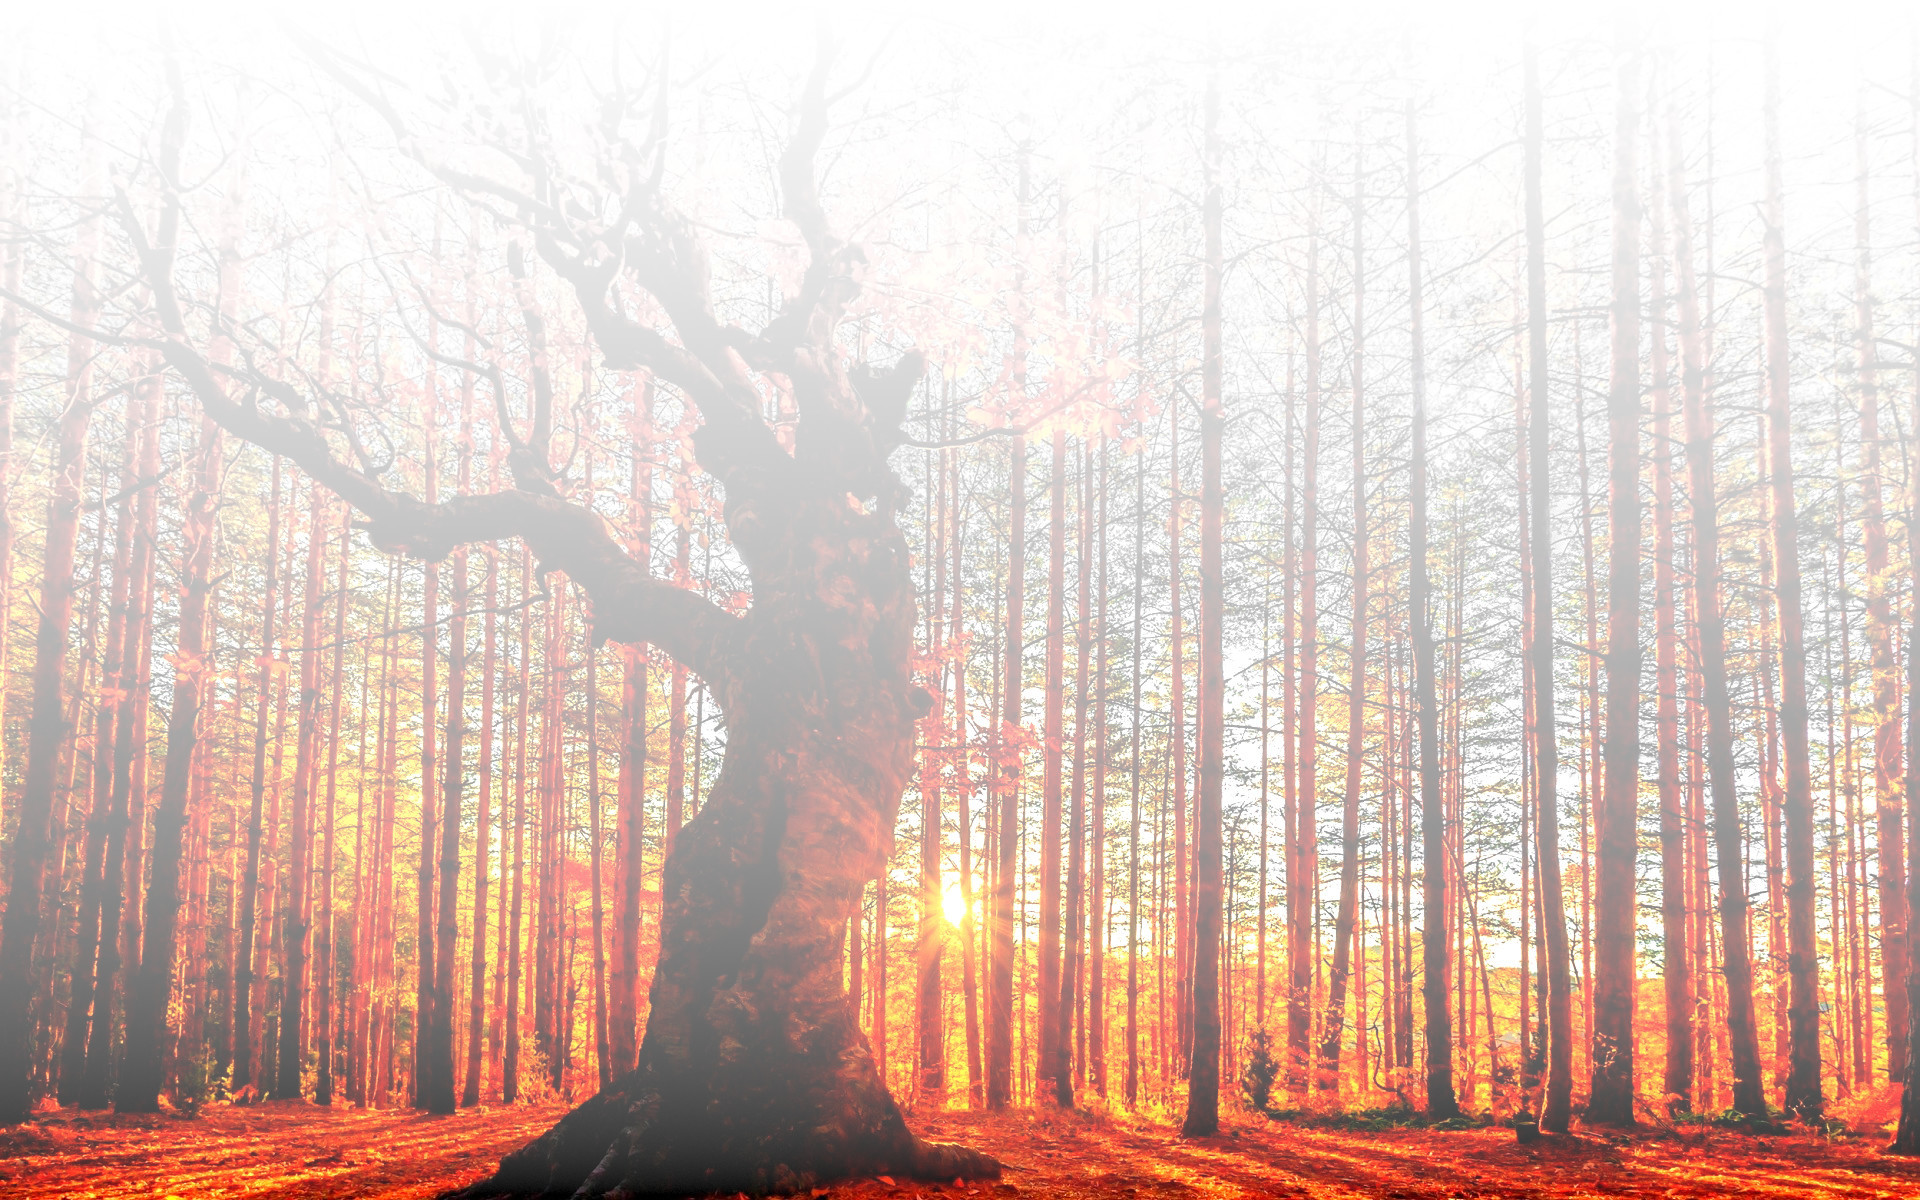
\includegraphics[width=\paperwidth]{forest-light}\end{minipage}}
\begin{frame}[c]
  \centering

  \bigskip
  \bigskip
  \bigskip
  \bigskip

  \scriptsize
  \textit{-- an invitation --}

  \setbeamercolor{block body}{bg=black!100}
  \begin{block}{}
    \centering\normalsize\color{white}
    \hil{On the scope of the \\ dynamical method in commutative algebra}
  \end{block}

  \bigskip
  \bigskip
  \bigskip
  \bigskip
  \bigskip
  \bigskip
  \bigskip

  \emph{Arbeitstagung Verona--München 2023} \\
  \bigskip

  Munich \\
  January 18th, 2022
  \bigskip

  Ingo Blechschmidt
  \par
\end{frame}}

\definecolor{mypurple}{RGB}{150,0,255}
\setbeamercolor{structure}{fg=mypurple}


\section{Dynamical algebra}

% \begin{document}

{\usebackgroundtemplate{\begin{minipage}{\paperwidth}\vspace*{5.95cm}
\includegraphics[width=\paperwidth]{fr1-lighter}\end{minipage}}
\begin{frame}{A primer to the dynamical method}
  \begin{varblock}{\textwidth}{}
    \justifying
    \textbf{Thm.}
    Let~$M$ be a surjective matrix with more rows than columns over a
    ring~$A$. Then~$1 = 0$ in~$A$.
  \end{varblock}

  \justifying
  \visible<2->{\emph{Proof.} \bad{Assume not.}}
  \visible<3->{Then there is~a \bad{maximal ideal} $\mmm$.}
  \visible<4->{The matrix is surjective over~$A/\mmm$.}
  \visible<5->{Since~$A/\mmm$ is a field, this is a contradiction to basic linear algebra.\qed}

  \only<3-5>{\bigskip\par\centering\scalebox{0.9}{\begin{tikzpicture}
    \node (0) at (0,1) {$(0) = \{0\}$};
    \node (1) at (0,5) {$(1) = \ZZ$};
    \node (2) at (-2,4) {$(2)$};
    \node [right of=2] (3) {$(3)$};
    \node [below of=2] (4) {$(4)$};
    \node [below of=2, xshift=0.7cm] (6) {$(6)$};
    \node [right of=3] (5) {$(5)$};
    \node [right of=5] (7) {$(7)$};
    \node [right of=7] (7d) {$\ldots$\phantom{(}};
    \node [right of=7d, xshift=3cm, yshift=-2cm] (max)
    {\vbox{\small\it maximal among the proper ideals \\ \medskip $\neg(1 \in
    \mmm)$ \\ \medskip $x \in \mmm \quad\vee\quad 1 \in \mmm + (x)$}};
    \node [below of=4] (8) {$(8)$};
    \node [right of=8, xshift=3cm] (8d) {$\ldots$};
    \draw (0) -- (8);
    \draw (0) -- (8d);
    \draw (0) -- (6);
    \draw (2) -- (1);
    \draw (3) -- (1);
    \draw (5) -- (1);
    \draw (7) -- (1);
    \draw (7d) -- (1);
    \draw (4) -- (2);
    \draw (8) -- (4);
    \draw (6) -- (2);
    \draw (6) -- (3);
    \draw [mypurple!30, thick, shorten <=-2pt, shorten >=-2pt, ->] (max) to [out=120, in=-30] (7d);
    \begin{pgfonlayer}{background}
      \draw[decorate, very thick, draw=mypurple!30]
        ($(2.south west) + (8pt, 0)$) arc(270:180:8pt) --
        ($(2.north west) + (0, -8pt)$) arc(180:90:8pt) --
        ($(7d.north east) + (-8pt, 0)$) arc(90:0:8pt) --
        ($(7d.south east) + (0, 8pt)$) arc(0:-90:8pt) --
        cycle;
    \end{pgfonlayer}
  \end{tikzpicture}}\par}
  \pause\pause\pause\pause\pause
  \bigskip

  \subhead{\hil{Three questions}}

  \begin{enumerate}
    \item \emph{Is there also a constructive proof?} \pause

    Yes, by completeness for coherent logic.
    \pause\medskip

    \item \emph{Do we know a constructive proof?} \pause

    \justifying
    Write~$M =
    \left(\begin{smallmatrix}x\\y\end{smallmatrix}\right)$. By surjectivity,
    have~$u, v$ with
    $
      u \left(\begin{smallmatrix}x\\y\end{smallmatrix}\right) = \left(\begin{smallmatrix}1\\0\end{smallmatrix}\right)
    $
      and
    $
      v \left(\begin{smallmatrix}x\\y\end{smallmatrix}\right) = \left(\begin{smallmatrix}0\\1\end{smallmatrix}\right)
    $.
    Hence $1 = (vy) (ux) = (uy) (vx) = 0$.
    \pause\medskip

    \item \mbox{\emph{Can the constructive proof be \hil{extracted} from the
    classical one?}}

    Yes, by the dynamical method (and others).
  \end{enumerate}
\end{frame}

\begin{frame}{The status of maximal ideals}
  \triang{} In \bad{classical mathematics}, every ring has a maximal ideal.

  \phantom{\triang} \small -- \emph{Zorn's lemma}
  \bigskip\pause

  \normalsize
  \triang{} Without \bad{Zorn}, every \bad{countable} ring has a maximal ideal.

  \emph{\phantom{\triang} \small\mbox{-- Iterative construction given enumeration~$x_0,x_1,\ldots$ [Krull 1929]:}}
  \small\begin{align*}
    \mmm_0 &= \{ 0 \}, &
    \mmm_{n+1} &= \begin{cases}
      \mmm_n + (x_n), & \text{if $1 \not\in \mmm_n + (x_n)$}, \\
      \mmm_n, & \text{else.}
    \end{cases}
    \intertext{\visible<3->{\mbox{\normalsize\phantom{\triang} \small\emph{-- Also constructively! [Krivine
    1996], [Berardi--Valentini 2004]}}}}
    \action<3->{\mmm_0 &= \{ 0 \}, &
    \mmm_{n+1} &= \mmm_n + (\underbrace{\{ x_n \,|\, 1 \not\in \mmm_n + (x_n)
    \}}_{\text{a certain subsingleton set}})}
  \end{align*}
  \pause
  \vspace*{-2em}
  \only<3>{\begin{columns}
    \begin{column}{0.3\textwidth}
      \begin{tikzpicture}
        \node (inner) at (17.3mm,-20mm) {\textit{``a bad joke''}};
        \path (0,0) pic{laurel-wreath};
      \end{tikzpicture}
    \end{column}

    \begin{column}{0.3\textwidth}
      \begin{tikzpicture}
        \node (inner) at (17.5mm,-18mm) {\vbox{\small\centering\textit{``non- \\informative''}}};
        \path (0,0) pic{laurel-wreath};
      \end{tikzpicture}
    \end{column}
  \end{columns}}
  \pause
  \vbox{\bigskip\phantom{\normalsize\triang \small\emph{--}} The quotient $A/\mmm$ is a residue field: noninvertible
  implies zero. \\
  \phantom{\normalsize\triang \small\emph{--}} $\neg(1 \in \mmm)$ \\
  \phantom{\normalsize\triang \small\emph{--}} $\neg(1 \in \mmm + (x)) \Longrightarrow x \in \mmm$}
\end{frame}
}

% \begin{document}

\begin{frame}{Forcing}
  \begin{itemize}
    \item[\triang] \hil{Forcing in commutative algebra}

    {\medskip\small
    \begin{tabular}{@{}p{2.0cm}l}
      $A \leadsto A[X]$ & adjoining an indeterminate \\
      $A \leadsto A[x^{-1}]$ & forcing an element to become invertible \\
      $A \leadsto A/(x)$ & forcing an element to become zero
    \end{tabular}}\bigskip

    \item[\triang] \hil{Forcing in classical set theory}

    {\medskip\small
    \begin{tabular}{@{}p{2.0cm}l}
      $V \leadsto V[G]$ & adjoining a generic filter of a forcing poset~$\PP$
    \end{tabular}}
    \small
    e.g. adding a cardinal between~$\aleph_0$ and~$\mathfrak{c}$, \\
    \phantom{e.g.} adding a random real, \\
    \phantom{e.g.} collapsing two cardinals, \ldots
    \normalsize
    \bigskip

    \item[\triang] \hil{Forcing in constructive mathematics}

    {\medskip\small
    \begin{tabular}{@{}p{2.0cm}l}
      $V \leadsto V^{\neg\neg}$ & forcing \textsc{lem} \\
      $V \leadsto \mathrm{Sh}(X)$ & adjoining a generic point of~$X$ \\
      $V \leadsto V[\TT]$ & adjoining a generic~$\TT$-model
    \end{tabular}}
  \end{itemize}
\end{frame}

\begin{frame}{Finite approximations to ideal objects}
  \fontsize{10pt}{12}\selectfont
  \begin{itemize}
    \item[\triang] Approximate \hil{maps}~$\NN \rightarrow X$
    by their finite prefixes.

    Given a finite list~$\sigma$, be prepared to \ldots

    \begin{enumerate}
      \footnotesize
      \item make it more defined: $\{ \sigma ::^r x \,|\, x \in X \}$
    \end{enumerate}
    \bigskip

    \item[\triang] Approximate \hil{enumerations}~$\NN \twoheadrightarrow X$
    by their finite prefixes.

    Given a finite list~$\sigma$, be prepared to \ldots

    \begin{enumerate}
      \footnotesize
      \item make it more defined: $\{ \sigma ::^r x \,|\, x \in X \}$
      \item ensure that a value~$x$ occurs: $\{ \sigma
      \concat \tau \,|\, \tau \in X^*, x \in \sigma \concat \tau \}$
    \end{enumerate}
    \bigskip

    \item[\triang] Approximate \hil{prime ideals} by finitely generated
    ideals.

    Given a f.g. ideal~$\aaa$, be prepared to \ldots

    \begin{enumerate}
      \footnotesize
      \item add the individual factors in case~$xy \in \aaa$: $\{ \aaa + (x), \aaa + (y) \}$
      \item collapse in case~$1 \in \aaa$: $\emptyset$
    \end{enumerate}
    \bigskip

    \item[\triang] Approximate \hil{local algebras} by finitely presented
    rings.

    Given a f.p. ring~$A$, be prepared to \ldots

    \begin{enumerate}
      \footnotesize
      \item invert the individual summands in case~$x+y$ is invertible in~$A$:
      $\{ A[x^{-1}], A[y^{-1}] \}$
      \item collapse in case~$1 = 0$ in~$A$: $\emptyset$
    \end{enumerate}
    \bigskip

%    \item[\triang] Approximate \hil{maximal ideals} by finitely generated
%    ideals.
%
%    Given a f.g. ideal~$\aaa$, be prepared to \ldots
%
%    \begin{enumerate}
%      \footnotesize
%      \item ensure maximality with respect to any~$x$: $\{ \aaa + (x) \} \cup
%      \{ \aaa + (u) \,|\, u \in A, u + vx = 1 \}$
%      \item collapse in case~$1 \in \aaa$: $\emptyset$
%    \end{enumerate}
  \end{itemize}
\end{frame}

\begin{frame}{The generic enumeration}
  For any monotone predicate~$P$ on finite lists,
  we inductively define what it means that

  \small
  \qquad
  \emph{no matter how a \hill{given list}~$\sigma$ evolves to a \hill{better
  approximation}~$\sigma'$, \\
  \qquad \hill{eventually}~$P(\sigma')$ will hold}\par

  \normalsize
  by the following clauses.
  \begin{enumerate}
    \addtocounter{enumi}{-1}
    \item \small If~$P(\sigma)$, then~$P \mid \sigma$.
    \item If~$P \mid \sigma ::^r x$ for all~$x \in X$, then~$P \mid \sigma$.
    \item If~$P \mid \sigma \concat \tau$ for all~$\tau \in X^*$ such that~$x
    \in \sigma \concat \tau$, then~$P \mid \sigma$.
  \end{enumerate}
\end{frame}

\end{document}
